\section{Sequential Circuits}

Figure 5.1 shows a block diagram of a sequential circuit. It consists of a combinational circuit to which memory elements are connected to form a feedback path.

\begin{figure}[H]
  \centering
  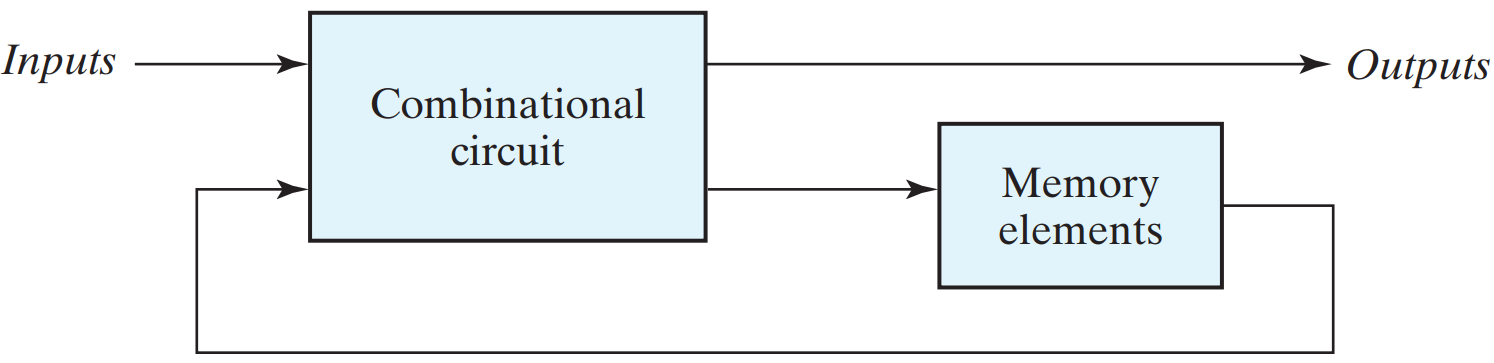
\includegraphics[width=\linewidth]{img/fig-5.1.png}
  \caption{Block diagram of sequential circuit}
  \label{fig:5.1}
\end{figure}

\textbf{A sequential circuit is specified by a time sequence of inputs, outputs, and internal states}.

There are two main types of sequential circuits, and their classification is a function of the timing of their signals:
\begin{itemize}
  \item A \textit{\textbf{synchronous} sequential circuit} is a system whose behavior can be defined from the knowledge of its signals at discrete instants of time.
  \item The behavior of an \textit{\textbf{asynchronous} sequential circuit} depends upon the input signals at any instant of  time \textit{and} the order in which the inputs change
\end{itemize}

A synchronous sequential circuit employs signals that affect the storage elements at only \textit{discrete instants of time}. Synchronization is achieved by a timing device called a \textit{clock generator}. The storage elements (memory) used in clocked sequential circuits are called \textit{flip-flops}.

The block diagram of a synchronous clocked sequential circuit is shown in 
Fig. 2.
\begin{figure}[H]
  \centering
  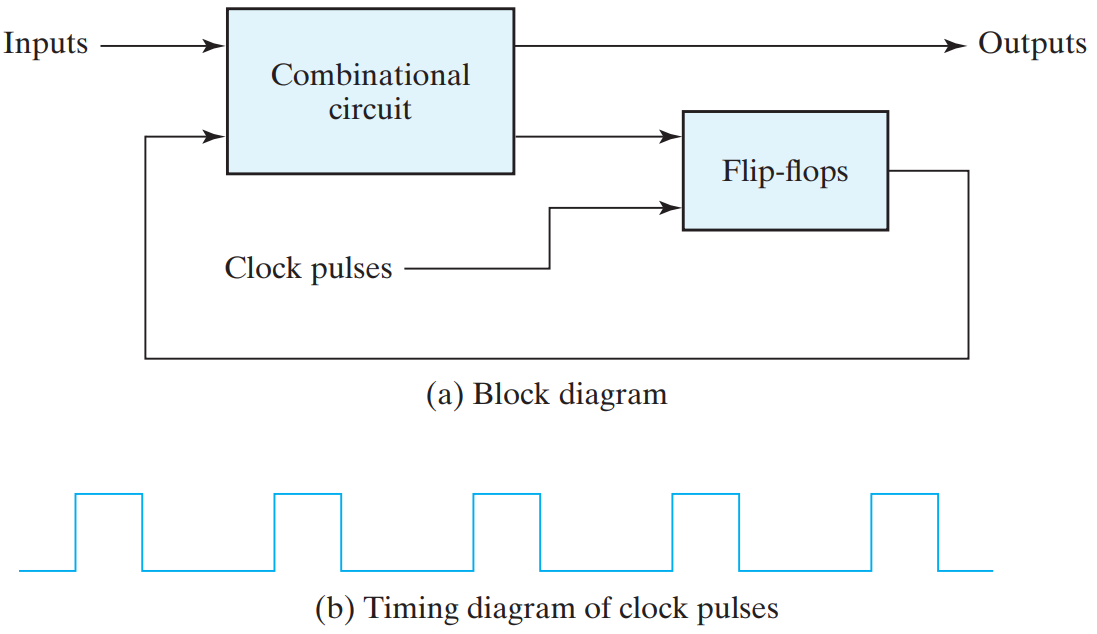
\includegraphics[width=\linewidth]{img/fig-5.2.png}
  \caption{Synchronous clocked sequential circuit}
  \label{fig:5.2}
\end{figure}

\begin{itemize}
  \item The \textit{outputs} are formed by a \textit{combinational logic function of the inputs to the circuit or the values stored in the flip-flops (or both)}. 
  \item The \textit{value that is stored in a flip-flop} when the clock pulse occurs is also determined by \textit{the inputs to the circuit or the values presently stored in the flip-flop (or both)}.
  \item The \textit{new value is stored} (i.e., the flip-flop is \textit{updated}) when a pulse of the clock signal occurs.
\end{itemize}

\textbf{Note:} The output of a combinational circuit depends on only the inputs to the circuit; the output of a sequential circuit depends on the inputs to the circuit and the present state of the storage elements.
